\chapter{System design}
\label{design}

We designed RAPID to fulfill the discussed system functionality and stylistic expectations discussed in Chapter~\ref{requirements}. This chapter focuses on our conceptual framework for moving toward those requirements; going from abstract to concrete, we also detail the process for converting these specifications to deployed source code---mapping broader logical entities and actions to specific modules, methods, and tables in Python and SQL.

Of further note, RAPID's design is mostly presented at the same level of abstraction as OGC's Abstract Specification---utilizing its standardized types and operators, just in an application-specific context. That is also to say, our model, with minimal modifications, could be implemented in any number of procedural programming languages and spatial DBMS. Our design decisions specifically aim for flexibility, clarity, and robustness, as there might be further development in the works.

One of our primary goals, here, is to spell out RAPID's data model and data flows. We describe basic storage and querying (as well as constraints)---continuing to build on the discussed standards---along with expected business rules and ancillary features. Among the high-level model descriptions, we share portions of source code and describe how we've used the Python-based Django web framework and PostGIS DBMS to implement RAPID.
% \footnote{The tradeoffs we considered in the design and implementation are a particular focus too. Because GIS data and software is so diverse---with many large and changing standards---we had to balance}


\section{Introduction}
We preface our contribution with a quick, helpful introduction to Django and related API work by Francis. We, additionally, describe our chosen pattern for cross-module method calls and finish by outlining a larger example we'll continue for the rest of the chapter.

\subsection{API design and capabilities}
In concert with Francis, and regarding the requirements from Chapter~\ref{requirements}, we defined several high-level API calls and activities for customer software (some of which are combined or broken into sub-steps):\footnote{The specific API syntax isn't essential to our discussion here. We list external DSS' primary tasks when using RAPID, but Francis provides more precise, developer-focused documentation~\cite{Francis}.}

\begin{enumerate}
  \item Creating DataLayer instances, including metadata.
  \item Importing GeoJSON and Shapefiles, adding their geospatial features to a designated DataLayer.
  \item Creating GeoView instances, including geometric boundaries and metadata.
  \item Choosing DataLayers for a GeoView.
  \item Browsing and filtering DataLayers, Features, and GeoViews.
  \item Setting permissions on DataLayers and GeoViews.
\end{enumerate}

Additionally, to manage permissions, each external system is assigned a unique and private API token that identifies them to RAPID. In the above API activities, the caller must include their secure token to be identified and provided properly-privileged data.

\subsection{Django usage with PostGIS}
\label{sec:prog}
To execute on RAPID's chosen functionality, Django (using a PostGIS database) quickly became a clear choice for our implementation framework, and we show how ordinary Python classes persist and are queried. These factors mainly influenced our decision:

\begin{enumerate}
\item Django's object-relational mapper lets us form database models quickly and use them wherever necessary in our Python codebase. Rather than crafting custom SQL queries, Django easily exposes tables and columns as classes and properties in Python.
\item Django is, sometimes, partially branded \textit{GeoDjango} and makes available a lot of GIS functionality---particularly in parsing and converting geometries.
\end{enumerate}

Referring to the technical advantages above, note further details and examples below. After this section, we won't dwell as much on Django implementation details: assume that future model creation and querying works in approximately the same form as these small tutorials.

\subsubsection{Django models}
Django creates and manages tables in our PostGIS database, mirroring them with classes defined in a \texttt{models.py} file. See how Django turns a class into a \texttt{CREATE TABLE} statement in SQL:

\begin{figure}
\begin{Verbatim}[samepage=true,baselinestretch=1,numbers=left,xleftmargin=12mm]
class Feature(models.Model):
    uid = models.TextField(unique=True, db_index=True)
    geom = models.GeometryField(null=True)
    bbox = models.PolygonField(null=True)
    properties = models.TextField(null=True)
    create_timestamp = models.TimeField(auto_now_add=True,
      null=True, db_index=True)
    layer = models.ForeignKey(DataLayer, null=True)
    hash = models.TextField(null=True, unique=True, db_index=True)
\end{Verbatim}
\caption{Feature class in models.py.}
\label{fig:feature}
\end{figure}

% archive = models.ForeignKey(Archive, null=True)

Many of the arguments in the fields are common database constraints:
\begin{itemize}
\item Setting \texttt{null} to \texttt{True} makes a column nullable.
\item Setting \texttt{auto\_now\_add} to \texttt{True} for a timestamp automatically populates it when inserting tuples.
\item Setting \texttt{db\_index} to \texttt{True} adds an index for that column to speed up matches. Note that, by default, all geometric fields are spatially indexed.
\item On foreign keys and other relations, the class type argument indicates the class or table that the model references.
\end{itemize}

Other field options exist for other purposes, which are described fully in Django's modeling documentation~\cite{Models}.  Note that, to ensure all database entries are fully and properly accounted for, Django adds an auto-incrementing \texttt{id} field to each model automatically, which acts as the primary key. The complete resulting GeoDjango SQL is available in Figure~\ref{fig:sql}.

% To expand on some database-specific nuances here: Django autogenerates surrogate primary keys business keys.

\begin{figure}
\begin{Verbatim}[samepage=true,baselinestretch=1,numbers=left,xleftmargin=12mm]
CREATE TABLE "rapid_feature" (
    "id" serial NOT NULL PRIMARY KEY,
    "uid" text NOT NULL UNIQUE,
    "geom" geometry(GEOMETRY,4326),
    "bbox" geometry(POLYGON,4326),
    "properties" text,
    "create_timestamp" time,
    "layer_id" integer REFERENCES "rapid_datalayer" ("id")
      DEFERRABLE INITIALLY DEFERRED,
    "hash" text UNIQUE,
    "modified_timestamp" time
);

CREATE INDEX "rapid_feature_uid_like"
  ON "rapid_feature" ("uid" text_pattern_ops);
CREATE INDEX "rapid_feature_geom_id"
  ON "rapid_feature" USING GIST ( "geom" );
CREATE INDEX "rapid_feature_bbox_id"
  ON "rapid_feature" USING GIST ( "bbox" );
CREATE INDEX "rapid_feature_create_timestamp"
  ON "rapid_feature" ("create_timestamp");
CREATE INDEX "rapid_feature_layer_id"
  ON "rapid_feature" ("layer_id");
CREATE INDEX "rapid_feature_hash_like"
  ON "rapid_feature" ("hash" text_pattern_ops);
\end{Verbatim}
\caption{CREATE TABLE statements generated by Django using the Python \texttt{Feature} class.}
\label{fig:sql}
\end{figure}

Our other classes defined in models.py---our whole data model---count on that same functionality to generate tables.

\subsubsection{Database interaction}
To create and store a class instance---a table entry---one can write the following (we use a mock Feature example):

\begin{Verbatim}[samepage=true,baselinestretch=1,numbers=left,xleftmargin=12mm]
new_feature = Feature(uid=12345,
  geom=`POINT(0 0)',
  properties=`{ "Description": "Test Feature" }')
new_feature.save()
\end{Verbatim}

Creating an in-memory object is equivalent to using any Python constructor (note the optional and named parameters compared to its definition). The \texttt{save()} method, to save the instance to our database, creates and executes a corresponding \texttt{INSERT} SQL statement.

Database queries mimick powerful \texttt{WHERE} clauses and joins in SQL. The static \texttt{filter} method on Django models returns a collection of selected objects, subject to the chosen parameters:

\begin{Verbatim}[samepage=true,baselinestretch=1,numbers=left,xleftmargin=12mm]
features = Feature.filter(uid=12345)
for feature in features:
    foo(feature)
\end{Verbatim}

Multiple \texttt{filter} calls can be chained to continue modifying the result set.\footnote{The \texttt{filter} method returns a QuerySet object that, generally, does not access the database until its results are evaluated. This means that, over time, filters can be changed on a result set and entries are queried as efficiently as possible \textit{only when needed}.} The below lookup finds Features with UIDs greater than 10000 (note the \texttt{gt} keyword) and \texttt{properties} strings containing ``Test''.\footnote{All the data operations in Django are much more complex than we can cover here. Refer to the official Django documentation for in-depth developer information.}

\begin{Verbatim}[samepage=true,baselinestretch=1,numbers=left,xleftmargin=12mm]
features = Feature.filter(uid__gt=10000)
features = features.filter(properties__contains=`Test')
for feature in features:
    foo(feature)
\end{Verbatim}

\subsubsection{Inter-module communication}
Having described Django's unique mechanisms and advantages, we now show our approach to passing messages between RAPID's persistence layer and the API modules. Francis organizes a \texttt{urls.py} file and a \texttt{views.py} file to parse incoming customer requests and generate suitable responses. Together, these define---precisely---how customers interact with our outside-facing REST API. Those responsibilities largely include extracting and transforming values from JSON (as well as creating sensible outputs).

For that code to retrieve and use database entries, Francis and I created an additional file---the intermediary \texttt{select.py}---to largely handle data management, utilizing the technical concepts previously outlined in this subsection. We map high-level API business logic to this file (like adding DataLayers to a GeoView) and also add three sets of functions for us us to easily add, retrieve, and delete customer-facing data: \texttt{create}, \texttt{get}, and \texttt{delete}. We name these \texttt{create\_feature}, \texttt{get\_feature}, \texttt{delete\_feature}, and so on with DataLayers and GeoViews. The \texttt{create} functions take in end users' parameters, performs any additional back-end processing and stores a newly-created object, returning its assigned UID to the caller. The \texttt{get} and \texttt{delete} functions take in a UID and fetch or delete (respectively) any corresponding database entry.

% \subsubsection{Summary}
% As a result, decoupled
% modify output and input without change the database
% the API relies on some idiomatic Django queries, so the database couldn't be swapped out, but it could be relatively easily.

\subsection{Chapter example}
To aid the remainder of this discussion, we introduce a small (but reasonable) example of RAPID in use. Consider a scenario with two pipeline operating companies that seek to
\begin{enumerate*}[label=\itshape\alph*\upshape)]
\item import and modify public \textit{and} private data and
\item create, share, and query GeoViews
\end{enumerate*}.

We imagine ABC Pipeline Co. and XYZ Operations both operate within San Luis Obispo (SLO) County, California, overseeing two pipelines: one in Paso Robles and one in Pismo Beach (note the county map in Figure~\ref{fig:county} and the city maps in Figures~\ref{fig:pismo}  and \ref{fig:paso}). The two companies cooperatively monitor and manage the section of pipeline in Pismo Beach, and XYZ Operations exclusively operates the section of pipeline in Paso Robles. For pipeline integrity management, each organization gathers and processes relevant datasets, intending to add them to RAPID (see Table~\ref{table:layers}). To easily monitor the data, ABC and XYZ create GeoViews for the two regions of interest.

\begin{table}[ht]

\begin{tabular}{ |l|l|l|l| }
% \multicolumn{4}{ |c| }{Example datasets} \\
\hline
Organization & Data & Covered region & Format\\
\hline
\multirow{2}{*}{ABC Pipeline Co.}
 & Traffic densities & SLO County & Shapefiles \\ \cline{2-4}
 & Construction equipment & Pismo Beach pipeline & GeoJSON \\ \hline
\multirow{2}{*}{XYZ Operations}
 & Rainfall & SLO County & GeoJSON \\ \cline{2-4}
 & Ground movement & Paso Robles pipeline & Shapefiles \\ \hline
\end{tabular}
\caption{Example pipeline operator datasets.}
\label{table:layers}
\end{table}

\begin{figure}
    \centering
    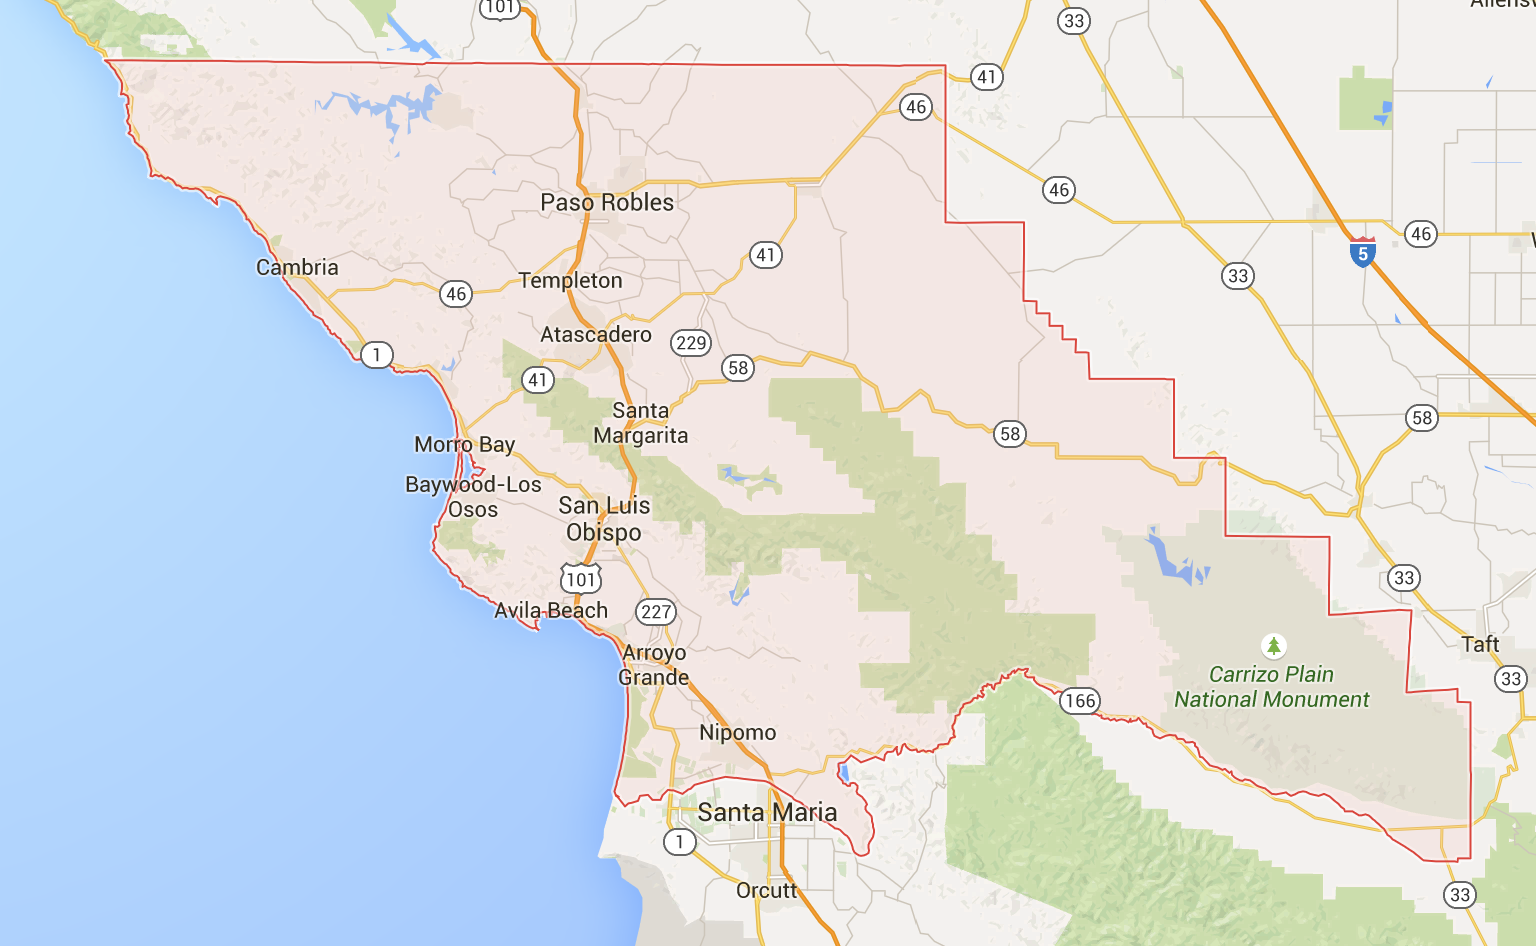
\includegraphics[width=0.84\textwidth]{figures/county.png}
    \caption{San Luis Obispo County lines. Note Paso Robles in the north. Pismo Beach (unlabeled) is between Avila Beach and Arroyo Grande}
    \label{fig:county}
\end{figure}

\begin{figure}
    \centering
    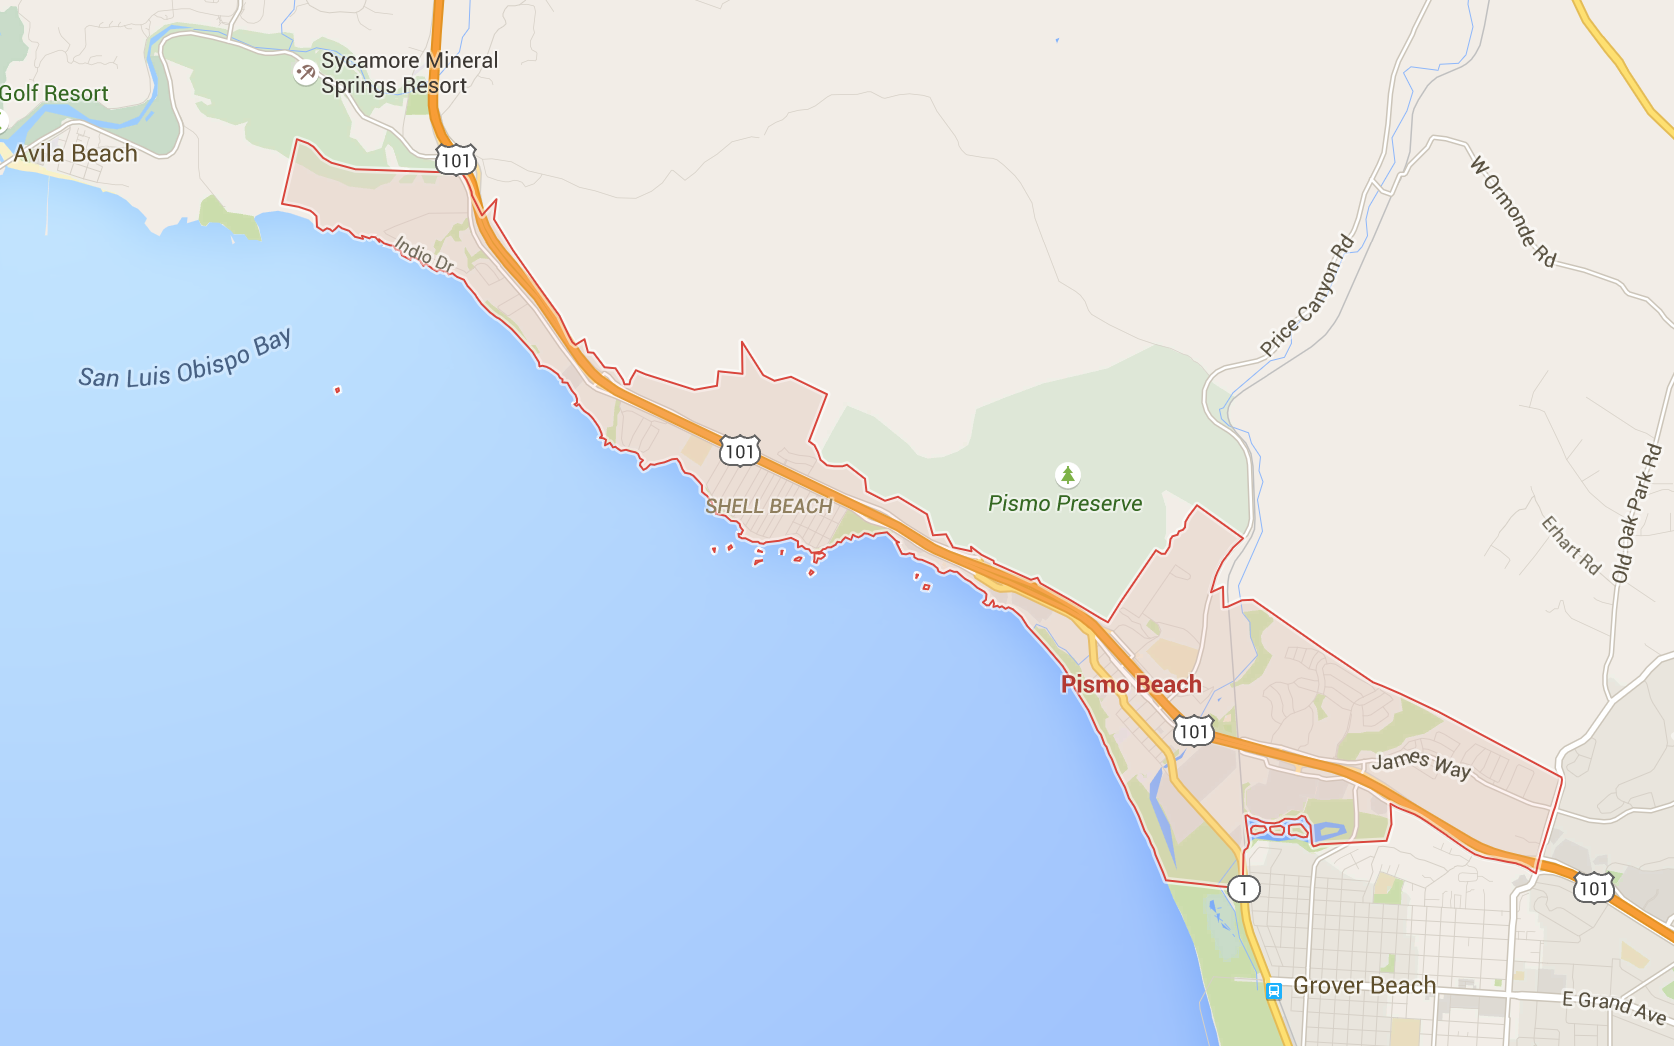
\includegraphics[width=0.87\textwidth]{figures/pismo.png}
    \caption{Pismo Beach city limits and pipeline region.}
    \label{fig:pismo}
\end{figure}

\begin{figure}
    \centering
    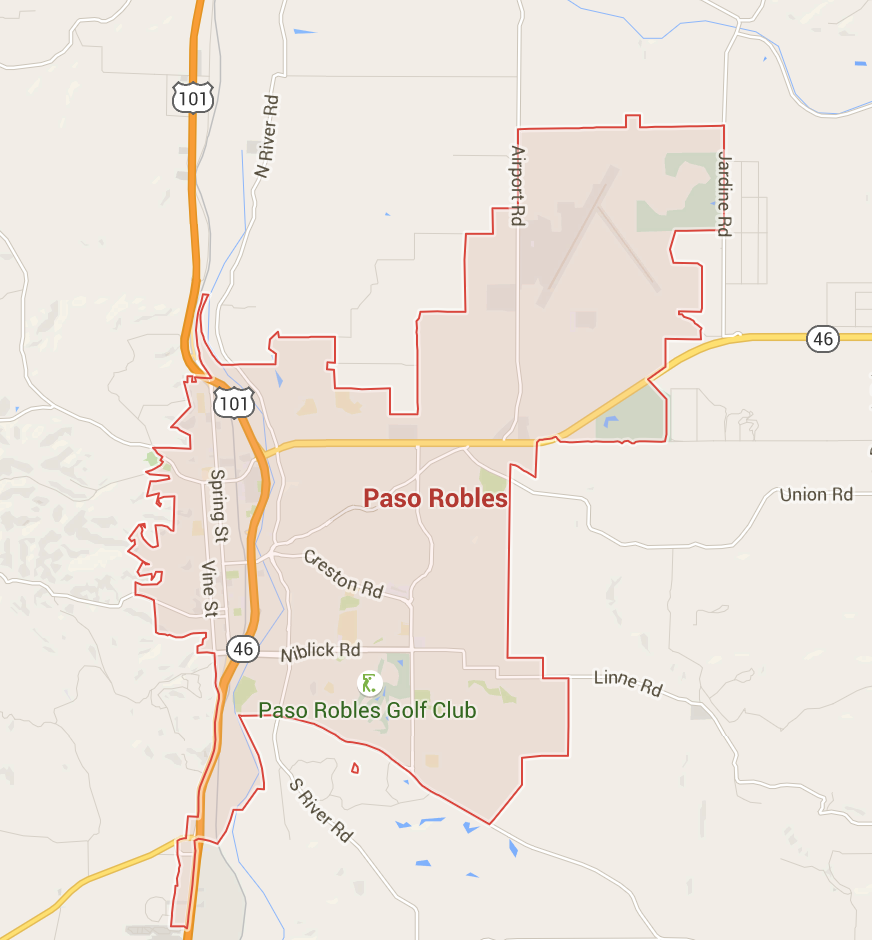
\includegraphics[width=0.55\textwidth]{figures/paso.png}
    \caption{Paso Robles city limits and pipeline region.}
    \label{fig:paso}
\end{figure}

The data from both organizations uses our permissioning system to allow shared, privileged access, as required by the business policies described below. Figure~\ref{fig:permissions} diagrams  
\begin{enumerate*}[label=\itshape\alph*\upshape)]
\item simple relationships between DataLayers and GeoViews and
\item the corresponding permissions setup for ABC Pipeline Co., XYZ Operations, and other RAPID users
\end{enumerate*}.

\begin{itemize}
\item As XYZ operates the Paso Robles pipeline on their own, they don't share the GeoView. The ground movement DataLayer is local and proprietary; they're sole Owner and Viewer. However, XYZ releases their rainfall DataLayer publicly, so that any RAPID user can view it.
\item Because ABC Pipeline Co. and XYZ Operations cooperate in the Pismo Beach pipeline region, ABC shares their relevant resources with XYZ: \begin{enumerate*}[label=\itshape\alph*\upshape)]
\item the county traffic DataLayer,
\item the Pismo Beach construction equipment DataLayer, and
\item the Pismo Beach GeoView
\end{enumerate*}.
\end{itemize}
 

\begin{figure}[ht]
    \centering
    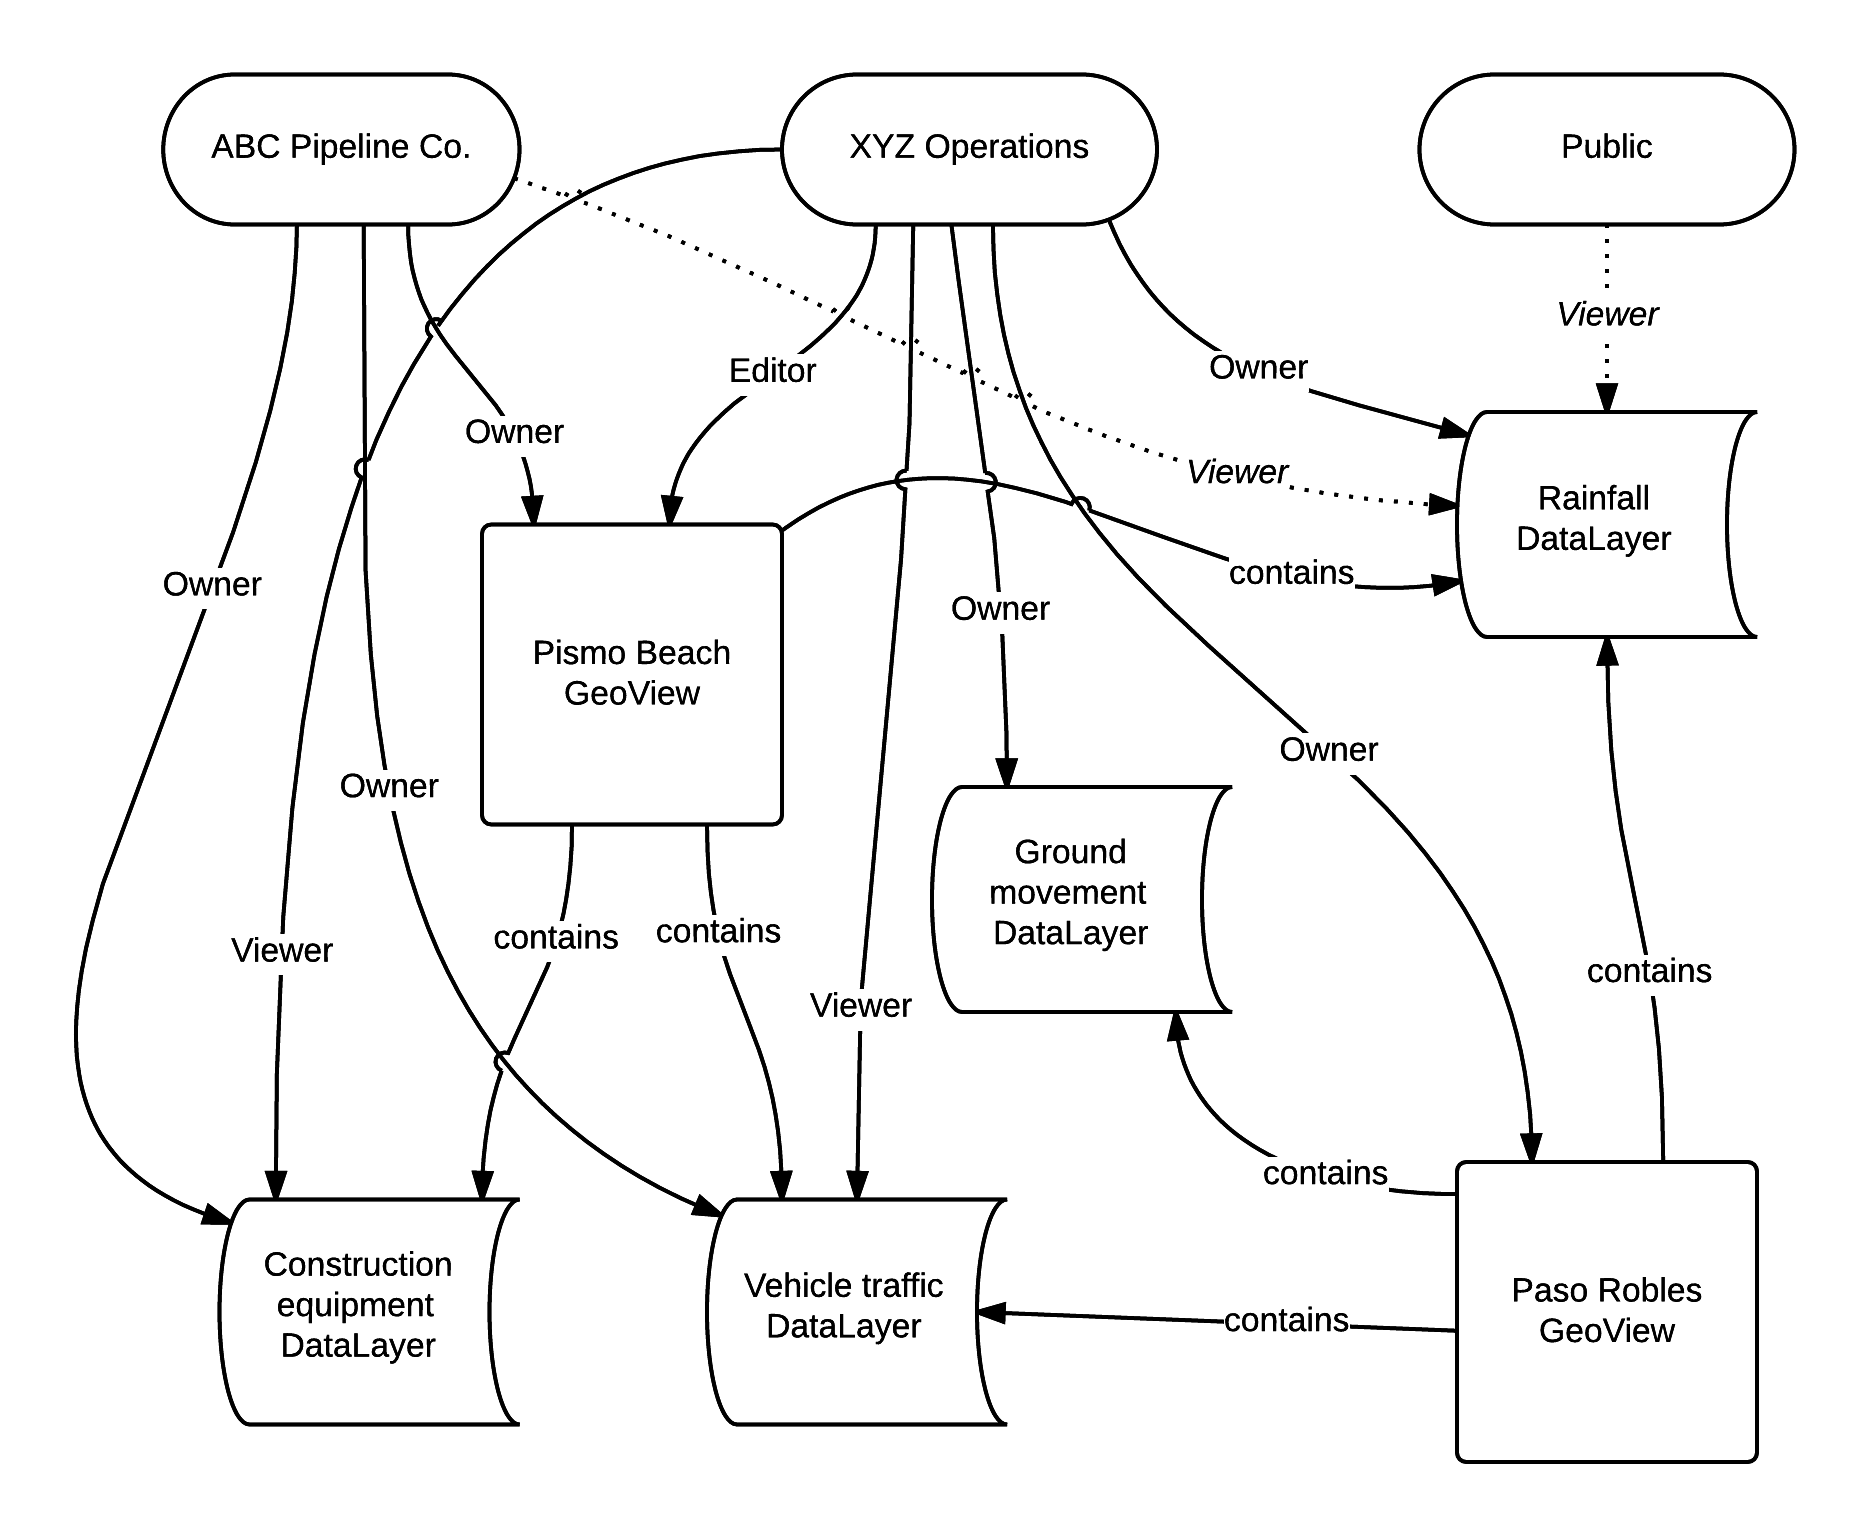
\includegraphics[width=0.99\textwidth]{figures/permissions.png}
    \caption{Example permissions setup between two organizations.}
    \label{fig:permissions}
\end{figure}

To slightly increase the complexity and realism of this example, we specify that the input formats begin as both GeoJSON and Shapefiles, and although ABC and XYZ review the same data for the same pipeline region, the groups use different DSS: ABC's only reads GeoJSON, and XYZ's only reads Shapefiles.

At a high level, with the above considerations, this scenario entails
\begin{enumerate*}[label=\itshape\alph*\upshape)]
\item setting up API tokens,
\item creating DataLayers,
\item importing GeoJSON and Shapefile features into DataLayers,
\item creating and querying GeoViews,
\item modifying permissions,
\item exporting data in GeoJSON and Shapefiles
\end{enumerate*}. Again note these are not always specific tasks for users---Francis describes those---but these end up being the most critical activities for our data model, described in the remainder of this chaper~\cite{Francis}. In other words, all of these can be accomplished by utilizing our models and writing queries with the techniques described in Section~\ref{sec:prog}, and following sections discuss specific class designs and source code that handle geospatial organization and querying. 

\begin{figure}[ht]
    \caption{Entity-relationship diagram for RAPID's three primary geospatial classes.}
    \centering
    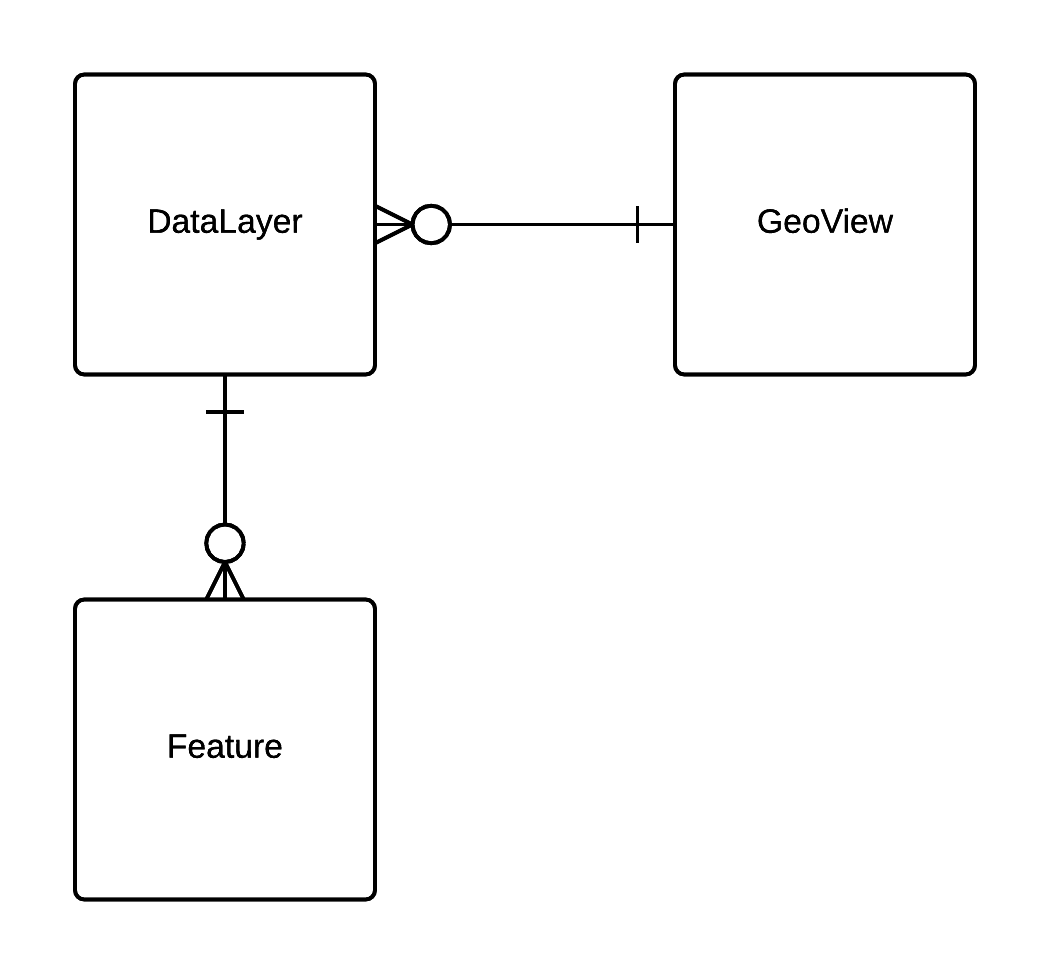
\includegraphics[width=0.5\textwidth]{figures/3er.png}
    \label{fig:3er}
\end{figure}

\section{Geospatial data modeling and organization}
Taken together, a small subset of RAPID classes enables structured data storage and retrieval for geographic features. In other words, these components could stand on their own, letting users browse and analyze geospatial objects (and groups of geospatial objects)---which fulfills our central database requirements. For the moment, we hold off discussing secondary functionality like permissioning, importing, and exporting data.

Figures~\ref{fig:feature},~\ref{fig:datalayer}, and~\ref{fig:geoview} show the relevant portions of our \texttt{models.py} file for the three models we've discussed throughout this paper. Figure~\ref{fig:3er}, shows a simple entity-relationship diagram to clarify the setup.

% archive = models.ForeignKey(Archive, null=True)

\begin{figure}
\caption{DataLayer class in models.py}
\begin{Verbatim}[samepage=true,baselinestretch=1,numbers=left,xleftmargin=12mm]
class DataLayer(models.Model):
    uid = models.TextField(unique=True, db_index=True)
    descriptor = models.TextField()
    properties = models.TextField(null=True)
    is_public = models.BooleanField(default=False)
\end{Verbatim}
\label{fig:datalayer}
\end{figure}

\begin{figure}
\caption{GeoView class in models.py}
\begin{Verbatim}[samepage=true,baselinestretch=1,numbers=left,xleftmargin=12mm]
class GeoView(models.Model):
    uid = models.TextField(unique=True, db_index=True)
    descriptor = models.TextField()
    geom = models.GeometryField(null=True)
    bbox = models.PolygonField(null=True)
    properties = models.TextField(null=True)
    layers = models.ManyToManyField('DataLayer', null=True)
\end{Verbatim}
\label{fig:geoview}
\end{figure}

\paragraph{Features}
We first describe the core makeup of \textit{features} in RAPID---that is, real geographic entities combined with other noteworthy indicators---and how they're presented to third parties. We saw in Chapter~\ref{background} that Geometry is the most generic and encompassing geospatial data type.\footnote{Remember that the Abstract Specification models these types hierarchically: a Polygon is a Polygon with holes, and a Polygon with holes is a Geometry, and so forth.} We also discussed that geospatial features correlate those mathematically-defined geometries with other descriptive attributes.

A RAPID Feature object is mostly a recreation of the geospatial features described in the Abstract Specification. There are some minor system-specific additions, but the purposes are similar enough that we borrow the terminology.

The Feature model comprises the following (with actual source code in Figure~\ref{fig:feature}):

\begin{description}
  \item[Geometry] \hfill \\
  A Geometry object represents the real-world footprint of the Feature (whether it's a Polygon, Line, Point, etc.). Functions from the OGC Standard can also be used to highlight various spatial characteristics like length, area, or circumference---calculations and descriptions people use everyday. Comparing two or more geometries (with the earlier-discussed relational operators) can reveal useful patterns, too.
   
   For simplicity, RAPID does not support elevations in a geometry. When importing Features, we only store the first two dimensions. This is usually fine for our pipeline operating partners: most relevant datasets are two-dimensional---the features are located on the Earth's surface (or at least within tens of feet).
   
   This missing third dimension is not related to the querying process (we never planned to allow Feature filtering based on height); it would only matter in data visualization or other analyses. In fact, three-dimensional geometry support is still rare in spatial DBMS (PostGIS is one of the only ones to actually support it). As an easy workaround on the user's end, the elevation could be ported rather easily to the Feature's properties, instead of residing in a Geometry.
  
  \item[Properties] \hfill \\
  Structured key-value stores are the norm for handling arbitrary GIS data, so an unlimited-length properties string bundles other relevant fields in a Feature. When shaping RAPID's usage style and conventions, we specifically wanted to support JSON as an intuitive data interchange format because our implementation leans on GeoJSON (and the REST API already parses JSON requests).
  
  The \texttt{properties} field introduces the ability to store and retrieve virtually any data for the Earth's surface (assuming it's serializable to JSON). Users that need extra functionality client-side can perform more advanced filtering and analysis with information besides just shape and location.
  
  \item[Unique identifier (UID)] \hfill \\
  We use a public, user-facing unique identifier (UID) for direct Feature lookups. While these could be any kind of unique value type, RAPID automatically generates textual UIDs upon Feature creation that are URL-safe and user-friendly (in that they're relatively short, using everyday numbers and letters).\footnote{We add UIDs to the three most prominent queryable models in RAPID---Feature, DataLayer, and GeoView---expecting that these are the objects under study and discussion. In that respect, the portability's very helpful.}\footnote{We coined this particular UID terminology for RAPID. An ``ID'' already gets used internally for back-end database work, and ``UUID'' (universally-unique identifier) is an existing standard for generating object identifiers~\cite{Leach}. Our UID makes use of the UUID standard behind the scenes, but they're not one and the same.} Because Features will often be retrieved using their UID, we add a database index for this field.
  
It's worth noting that our UIDs are generated randomly (with a secure random number generator) and end up being 22 bytes. An integer identifier would be reasonable too (especially with some slight indexing efficiencies over a longer string), but random strings won out:
  
  \begin{itemize}
  \item Features are the most numerous object type in RAPID. While we wouldn't expect to easily max out a 32- or 64-bit number, 22 bytes erases any worry of integer overflow when deployed over a wide area and many years.\footnote{The same argument could be made with fewer bytes: the library we're using happens to use 22.}
  \item We don't want identifiers to indicate ordering, magnitude, or chronology for Features: the UID should look more like a hash, as proximate integers could otherwise imply a relevant or analyzable relationship.
  \item Following that logic, a random string is helpful from a security standpoint. One organization could theoretically share UIDs for all their classified Features in the open, but no one else would be able determine how new, old, or similar they are through the UID. An incrementing counter could otherwise hint at those characteristics.
\end{itemize}
  
\item[Bounding box] \hfill \\
  It's somewhat common for GIS features to include a bounding box attribute---defining the minimally-bounding rectangle for the geometry. The small number of coordinates in a bounding box can estimate and rule out results in spatial functions more quickly than the ``true'' geometry.

  RAPID does not currently use bounding box checks (but they could be useful in the future, pending performance tests). However, bounding boxes are an important GIS topic in Simple Features Access, so we store them anyway~\cite{SFA}.
  
\item[Timestamp] \hfill \\
RAPID stores timestamps with Features---a filterable attribute when querying GeoViews---to indicate their relevance in time.

In a technical regard, \texttt{timestamp} is unremarkable, as it's simply another attribute to filter (as a range) when querying Features. However, as discussed in Chapter~\ref{background}, trend-watching is particularly useful and needed in GIS work. This timestamp lets pipeline operators and DSS find data that \begin{enumerate*}[label=\itshape\alph*\upshape)]
\item is most recent and applicable or
\item relevant for historical analyses
\end{enumerate*}.
  
\item[DataLayer foreign key] \hfill \\
A foreign key references the Feature's DataLayer---the DataLayers's \texttt{id}. Note that this is a many-to-one relationship (and the primary reason the relationship is directed from Feature to DataLayer). In other words, a Feature always has access to its DataLayer.

\textbf{Implementation note.} This one-way relationship, however, doesn't preclude us from traversing the relationship in the other direction---seeing all the Features for a DataLayer. That alternative action is common enough, and Django makes the querying easy: 

\begin{Verbatim}[samepage=true,baselinestretch=1,numbers=left,xleftmargin=12mm]
features = layer.feature_set
\end{Verbatim}

Even though a \texttt{feature\_set} isn't explicitly defined for a DataLayer, Django adds the property implicitly and handles the reverse lookup of the primary keys behind the scenes.

\end{description}

\paragraph{DataLayer}
DataLayers exist to usefully store multiple similarly-structured Features. Although there's a notion of layering in OGC standards, RAPID diverges from any of their detailed considerations and only keeps the spirit of categorization---hence the rename~\cite{AbstractSpecFaq,SFA,WFS}.

While RAPID doesn't enforce a consistent structure on properties, we'd expect them to be similar within a DataLayer so that they can be analyzed consistently. Although a misnomer, a DataLayer's Features might be imagined as \textit{instances} of the layer descriptor (see below), if they have similar schemas.

DataLayers start out with these fields:

\begin{description}

\item[UID] \hfill \\
DataLayers use the same UID construction as Features. While the larger string size isn't as necessary for the number of DataLayers as it is with Features---their count will never be the same order of magnitude---we keep the same setup for consistency. We could partially truncate the UID for DataLayers (and GeoViews) if we had to be extra concerned about it.

\item[Descriptor] \hfill \\
As a simple user-friendly and -facing title for DataLayers, we include a short Descriptor text field. The Descriptor labels the set of contained Features; ``Earthquake'' and ``Construction equipment'' are reasonable examples.

\item[Properties] \hfill \\
To mirror the properties capabilities in Features, we store JSON metadata in DataLayers (and leave it up to third parties to define the fields). Use of the metadata is optional, but it sometimes includes important documentation for Features' properties.

\item[Public flag] \hfill \\
When creating a DataLayer, we ask users to specify if it's a \textit{public} DataLayer, which anyone is allowed to view. For DataLayers that should be widely-accessible, this removes the inconvenience of adding a lot of Viewers manually. The original creator retains ownership and can continue to add other Owners and Editors as necessary (described later in this chapter).
  
\end{description}

 We haven't carried out performance testing to determine the tradeoffs, but we specifically chose \textit{not} to include bounding boxes on DataLayers, even though there \textit{could} be significant efficiency improvements to explore: one check with a DataLayer bounding box could avoid costly comparisons against thousands (or millions!) of Features. It'd be somewhat more complex, however, to keep the bounding dimensions up to date: as soon as Features change within a DataLayer, the bounding box must be recalculated.\footnote{The system design could have been set up to incorporate this, and there's an obvious place in the implementation to include the code, but it's outside our scope of work.}

\paragraph{GeoViews.}
It's possible (and reasonable) to retrieve all Features for a given DataLayer, but a more common and interesting use case lets users narrow the scope to a more precise and helpful dataset. This is shown explicitly with GeoViews---a way to retrieve data from combined DataLayers for a particular area. We, in fact, mostly expect applications to query GeoViews during daily operation---not DataLayers or Features---because they encompass a more complete study-able concept.

To elaborate, a GeoView includes 
\begin{enumerate*}[label=\itshape\alph*\upshape)]
\item one or more DataLayers and
\item a Geometry for a region of interest
\end{enumerate*}. RAPID saves which DataLayers are added to the view; when the GeoView is queried, Features from those DataLayers are returned to the requestor if they encroach on the chosen Geometry. GeoViews are rather analogous to ordinary SQL views (bringing about the name). They could even be implemented as them (aside from metadata), if so chosen.

To accommodate this functionality in the API, we define the GeoView model with these attributes:

\begin{description}

\item[DataLayer collection] \hfill \\
Each GeoView has a collection of the DataLayers to retrieve Features from. Users can add DataLayers to GeoViews (and remove them), so at run-time, their chosen DataLayers are searched.

\item[Geometry] \hfill \\
To indicate a specific physical location to query within or around, GeoViews include an assignable Geometry field. Early in requirements gathering, it was a forgone conclusion that GeoView Geometries narrow DataLayers to their specified region. That implied using the \texttt{Intersects} boolean relational operator so that all Features within or encroaching on a region are available. On the other hand, as RAPID's implementation progressed and API calls were tested, we noticed the value in supporting several of the Abstract Specification's spatial operators.

As such, \texttt{Intersects} is left as the default, but we also let callers to this interface choose \texttt{Contains} or \texttt{DWithin}. \texttt{Contains} produces of subset of the results of \texttt{Intersects}; the difference is that ``contained'' Features are \textit{fully} contained within the Geometry and cannot merely be overlapping the border. The \texttt{DWithin} operator produces a superset of Features from the \texttt{Intersects} results; the difference is Features within a certain distance of the Geometry are also selected. \texttt{DWithin} could highlight nearby Features that are still relevant (or that may be relevant in the future).

\item[Bounding box] \hfill \\
Again, pending performance tests, GeoView bounding boxes could prove to better our speeds, but they aren't currently set or used in our queries. We don't have the same concerns with bounding box consistency as we do with DataLayers, however, because there's only one geometry associated with the object.

\item[UID] \hfill \\
This identifier for GeoView rounds out our use of UIDs, included for the same reasons discussed in Features and DataLayers.

\item[Descriptor] \hfill \\
It makes sense for GeoView instances to have a user-friendly name to encompass their purpose---possibly shuffled among other GeoViews. An example we've seen would include ``Pismo Beach Pipeline.''

\item[Properties] \hfill \\
Included for the same reason in DataLayers, a properties field stores any desired metadata. In the case of GeoViews, users may want to provide detailed explanations on why the DataLayers are relevant or what different values indicate.

\end{description}

\textbf{Implementation note.} Django simply presents many-to-many relationships as collections in each model. Take the following example, where a DataLayer is added to a GeoView:

\begin{Verbatim}[samepage=true,baselinestretch=1,xleftmargin=12mm]
geoview.layers.add(layer)
\end{Verbatim}

Behind the scenes, Django creates and populates a junction table, mapping DataLayers to GeoViews (using their auto-generated primary keys).

\textbf{Example.} Instances of Features, GeoViews, and DataLayers.

\section{Importing and exporting data}
We can now describe how data is added to RAPID---how Features are ``imported'' from geospatial file formats---which might occur on-demand from API requests or at regular intervals automatically. We also take the opportunity to describe the export process.\footnote{Note that this only goes as far as to say how Features become and are converted from geospatial formats. The REST API itself includes other metadata and formatting in its requests and responses; the serialized geospatial file may be embedded in a larger JSON object~\cite{Francis}.} As we discussed in Chapter~\ref{design}, RAPID must read from and write to a variety of geospatial file formats (GeoJSON and Shapefiles at first). Here, we note how a user specifies a file and file type, and the generic process RAPID uses to parse and save Features. Although our requirements do specify GeoJSON and Shapefile support, we know other parsing capabilities may be required soon. As such, we've structured the objects and interfaces so that additional file formats will be easily importable at another time.\footnote{In general, we've looked to future-proof these high-level interfaces so that they're more dependent on the Abstract Specification than any one format or library.}

\subsection{Importing files}
The multiplicity of spatial and geographic file specifications is mirrored by the number of options in parsing, writing, validating, and transforming them. Some tools are easier to use than others; some support files that others don't. Some spatial DBMS will even handle encoding and decoding of popular formats natively. Therefore, we prioritize flexibility in the architecture for importing files and set up a pattern and process for consistent conversion.
 
In an \texttt{import.py} file, we add high-level file retrieval and parsing functionality, letting the API designate a file type and file location to import. As currently implemented, RAPID can parse GeoJSON and Shapefiles from a URL or on-disk file path. Once the file content is available, it's fed into a parser.\footnote{GeoJSON is an ordinary text-based file format, but as we discussed in Chapter~\ref{background}, Shapefiles are made of up multiple files, so they're transferred and stored as \texttt{.zip} files. Before parsing the extracted files, RAPID unzips this file.}

At a minimum, the parsing utilities and methods must extract geometries and key-value properties from the specified file content. With those available, they can be passed (along with the chosen DataLayer's UID) to our \texttt{create\_feature} function to handle final processing and . The property dictionary is converted to JSON; the geometry must end up in GeoJSON or WKT.\footnote{We don't dive into intricacies of file parsing and validation: official documentation and other tutorials provide the most accurate and proper guidelines. For example, we use GEOS for spatial data structures and operations, and python-geojson and PyShp for reading GeoJSON and Shapefiles~\cite{1,2,3}.}

Because multiple files can be added to one DataLayer, duplicate Features could be encountered; however, we need to eliminate redundancies so that these aren't interpreted as discrete entities. To address this, we add a hash value---a digest of the Feature---with the constraint that it is unique per DataLayer. In other words, any new features with precisely the same geometry and properties as an existing feature are disregarded.


\subsection{Exporting Features}
Exporting retrieved Features (maybe from queried GeoViews) works similarly to file importing (except in reverse), but it is primarily in the realm of Francis's API work~\cite{Francis}. To summarize, these are some of the critical steps and considerations:

\begin{itemize}
\item Blah 1
\item Blah 2
\end{itemize}

\section{Permission management}
Chapter~\ref{requirements} laid out permissioning capabilities for RAPID DataLayers and GeoViews. That functionality is enabled by adding several components. The entity-relationship diagram in Figure~\ref{fig:er} builds on the diagram in Figure~\ref{fig:3er}, showing the additional classes that make this an operational multi-tenant system.

\begin{figure}[ht]
    \centering
    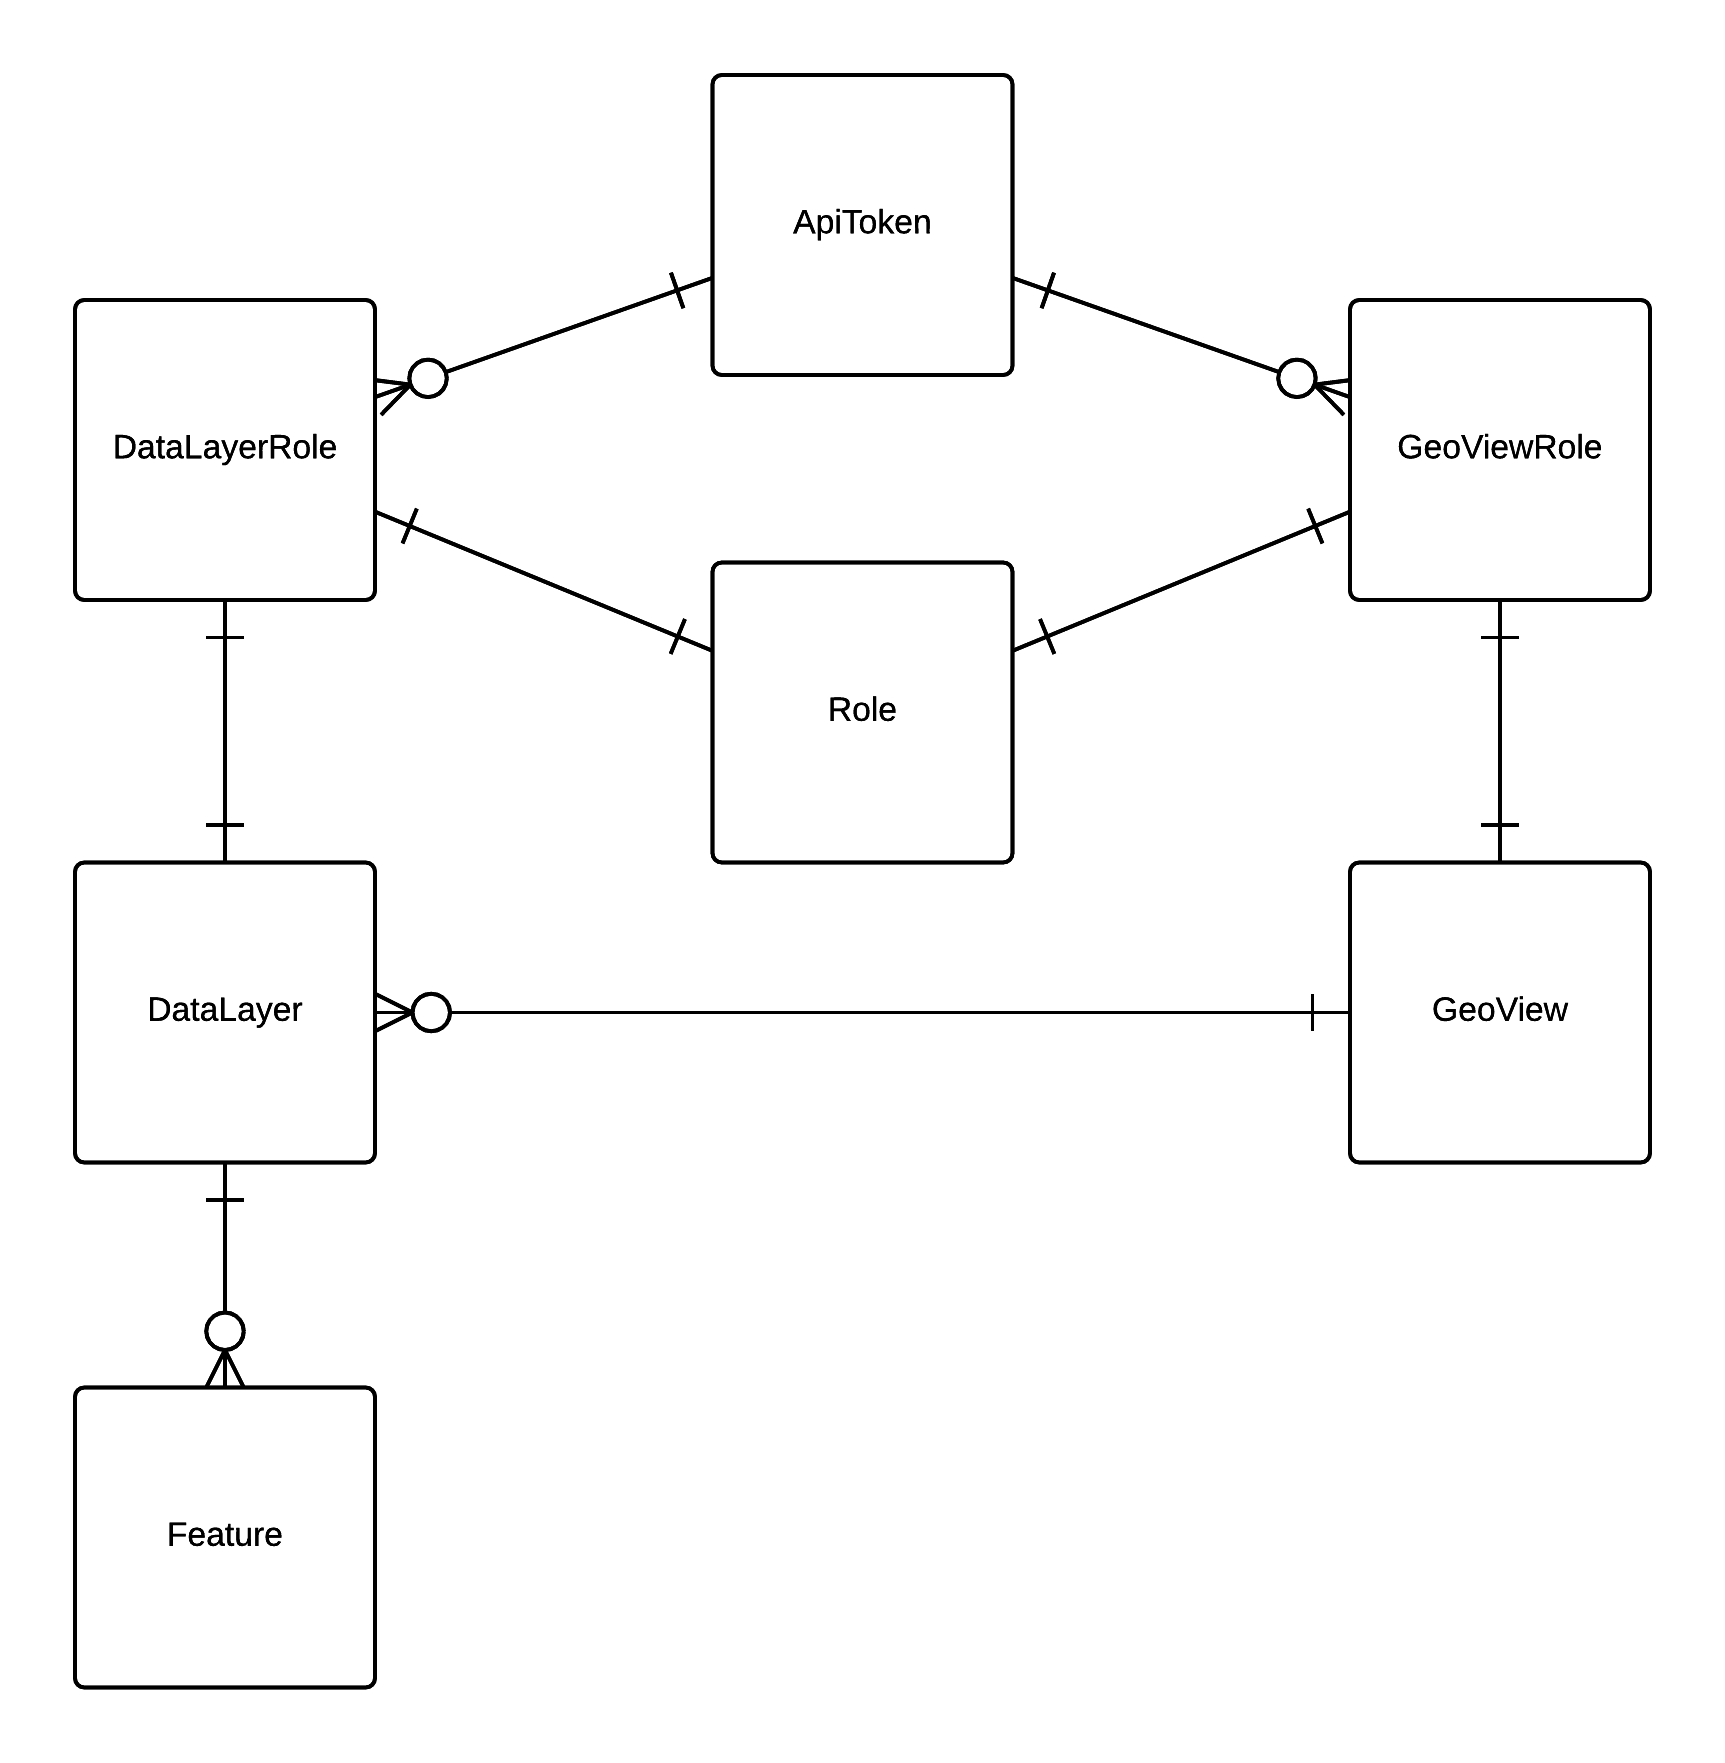
\includegraphics[width=0.99\textwidth]{figures/er.png}
    \caption{Entity-relationship diagram for RAPID's main conceptual data model, with permissioning capabilities.}
    \label{fig:er}
\end{figure}

\subsubsection{Role enum}
We add an enum, Role, to define the three available permission roles for RAPID data:
\begin{itemize}

  \item Owner
  \item Editor 
  \item Viewer
  \end{itemize}

Again recall that, on a daily basis, in-operation software is RAPID's end user: \textit{people} aren't necessarily Owners, Editors, or Viewers of data. We instead distribute API tokens that have assignable roles on each DataLayer and GeoView, and any system using that token has a uniform view of RAPID's resources.

\subsubsection{ApiToken}
The simple ApiToken model associates a friendly name (used as an identifier for administrative purposes) with a cryptographically-secure, randomly-generated key that grants resource access. When API requests come \textit{with} a token, RAPID knows who or what is requesting data and can return an appropriate set of results.


\begin{figure}
\begin{Verbatim}[samepage=true,baselinestretch=1,numbers=left,xleftmargin=12mm]
class ApiToken(models.Model):
    key = models.TextField(unique=True, db_index=True)
    descriptor = models.TextField(unique=True)
    issued = models.TimeField(null=True, auto_now_add=True)
\end{Verbatim}
\label{fig:apitoken}
\end{figure}

\begin{description}
\item[Name] \hfill \\
We require a friendly public name to identify this token. This can be used when choosing and assigning permissions for RAPID's other managed tokens.

\item[Key] \hfill \\
Upon creating an ApiToken and giving it a name, the system creates a long, random, URL-safe hash value to use as a password for sharing and accessing privileged data. When performing access-dependent API activities, the caller uses the (unguessable) token to show that they have the correct permissions, and RAPID checks the key against its internal records (the DataLayerRole and GeoViewRoles below).\footnote{While this setup is an accepted basis for web-based API security, RAPID should see an audit before storing truly classified data. For example, any other security measures are for naught if HTTPS is not enabled on the production server~\cite{Stormpath,Palmer}. }

\item[Timestamp] \hfill \\
Although our work is not focused on the security aspects of RAPID, we define and assign a creation timestamp for each token so that expiration or renewal policies can be implemented by future contributors.

\end{description}
To track newly-assigned permissions on DataLayers and GeoViews, we create DataLayerRole and GeoViewRole models, associating an ApiToken with a DataLayer or GeoView and specifying the particular role.


\begin{figure}
\begin{Verbatim}[samepage=true,baselinestretch=1,numbers=left,xleftmargin=12mm]
class GeoViewRole(models.Model):
    token = models.ForeignKey(ApiToken)
    role = enum.EnumField(Role)
    geo_view = models.ForeignKey(GeoView)
\end{Verbatim}
\label{fig:geoviewrole}
\end{figure}

\subsubsection{DataLayerRole and GeoViewRole}
\begin{description}
\item[ApiToken foreign key] \hfill \\
Specifies the ID of the ApiToken that has resource access.

\item[DataLayer or GeoView foreign key] \hfill \\
Specifies the ID of the DataLayer (if a DataLayerRole) or GeoView (if a GeoViewRole) to assign permissions to.

\item[Role enum] \hfill \\
The Role enum specifies the level of access this setup grants for the token on the chosen object.
\end{description}

% Could add user support to tokens down the road

\textit{[Integrate examples with ABC and XYZ's permissioning setup, showing specific roles and API tokens.]}


\label{design_srid}
